\chapter{Implementación del primer incremento}
\section{Lenguajes y herramientas}
La interfaz utiliza TypeScript con React. La API utiliza JavaScript ESM ejecutado con Node.js 24 y Express 5. Zod valida entradas con mensajes en español; SQLite persiste datos mediante el módulo \texttt{node:sqlite}; Node Test Runner y Supertest verifican la API, y Playwright automatiza flujos de navegador Chrome.

Las versiones resueltas en esta construcción son Express 5.3.0, React 19.3.1, Zod 4.6.7, Vite 8.3.8 y TypeScript 7.0.2. La fuente reproducible es \path{package-lock.json}; estas versiones no estaban presentes en la base documental inicial. El entorno inspeccionado ofrece Node 24.16.0. La documentación oficial describe los requisitos y las funciones de Express, Vite y SQLite \cite{express5,vite,nodesqlite}.

\section{Archivos y comunicación entre módulos}
\begin{longtable}{P{5.7cm}P{7cm}}
\caption{Responsabilidades de archivos principales}\\
\toprule Archivo o carpeta & Responsabilidad \\ \midrule
\endfirsthead
\toprule Archivo o carpeta & Responsabilidad \\ \midrule
\endhead
\path{src/App.tsx} y módulos de interfaz & Formularios y vistas de acceso, panel, usuarios, roles y capacitaciones \\
\path{src/api.ts} & Solicitudes a la API y tratamiento de errores de contrato \\
\path{server/index.js} & Inicio del proceso y configuración del entorno \\
\path{server/app.js} & Composición de middleware, rutas y manejo final de errores \\
\path{server/routes/auth.js} & Inicio, consulta y cierre de sesión \\
\path{server/routes/users.js} & Entradas HTTP de usuarios y roles \\
\path{server/routes/trainings.js} & Entradas HTTP de capacitaciones y consultas iniciales \\
\path{server/services/user-service.js} & Reglas de usuarios, roles e integridad administrativa \\
\path{server/services/training-service.js} & Validación de planificación y transiciones \\
\path{server/security.js} & Hashing, sesiones, CSRF y autorización \\
\path{server/db.js} & Conexión, migraciones y transacciones \\
\path{server/migrations/001_initial.sql} & Esquema inicial con restricciones persistentes \\
\path{server/seed.js} & Datos ficticios de demostración y configuración de cuenta inicial \\
\path{tests/api.test.js} & Casos HTTP de usuarios, roles y capacitaciones \\
\path{tests/security.test.js} & Sesión, CSRF, límites y controles de privilegios \\
\path{tests/persistence.test.js} & Reapertura de base, rollback y migraciones incrementales \\
\path{tests/ui.spec.ts} & Flujos de navegador automatizados; resultados separados de API \\
\bottomrule
\end{longtable}

El formulario no ejecuta SQL. Envía JSON a una ruta, que valida y delega al servicio. El servicio aplica reglas y coordina persistencia. La respuesta informa éxito después de confirmar la operación. Una falla de integridad no debe dejar la auditoría o una asignación de rol parcialmente guardadas.

\section{Autenticación, usuarios y roles}
HU-16 habilita el flujo protegido de HU-01 y HU-02. El login verifica la contraseña y el estado activo; la cookie de sesión y el token CSRF acompañan solicitudes posteriores. Un usuario autenticado no recibe automáticamente permiso administrativo.

El registro de usuario admite nombres, apellidos, correo, documento opcional, área textual, especialidad, estado y roles. La contraseña solo es obligatoria al crear y nunca se devuelve en consultas. Una edición debe conservar administración activa y rechazar duplicados. La asignación de roles exige \texttt{roles.manage}; delegar solo \texttt{users.manage} no permite crear cuentas privilegiadas ni editar las que tengan gestión de usuarios o roles. La gestión de roles permite consultar el catálogo y cambiar permisos de roles no administrativos con autorización.

\section{Registro y edición de capacitaciones}
HU-03 y HU-04 usan una capacitación con código, título, descripción, periodo, horario, modalidad, ubicación, capacidad y estado. El responsable procede de la sesión autenticada; no se confía en un identificador privilegiado enviado por el navegador. El instructor es opcional y, cuando se informa, debe ser un usuario válido con el rol correspondiente.

La lista permite consulta y filtros. La creación admite estados iniciales definidos y la edición comprueba el grafo de transiciones. El control de capacidad V1 valida un entero entre 1 y 10\,000; aún no prueba un flujo de ocupación de cupos con inscripciones, porque ese módulo está pendiente. El instructor consulta únicamente capacitaciones asignadas. El participante no recibe filas ajenas mientras no exista el módulo de inscripciones.

\section{Fragmentos del código real}
Los siguientes listados se leen directamente del código del repositorio. Si se prepara una copia autónoma para Overleaf, el script incluido copia esos mismos archivos y registra sus hashes. No se presenta pseudocódigo como una captura de implementación.

\fragmentocodigo{server/db.js}{1}{45}{Inicio del módulo real de persistencia y migraciones}
\fragmentocodigo{server/security.js}{1}{55}{Inicio del módulo real de seguridad}
\fragmentocodigo{server/services/training-service.js}{1}{60}{Inicio del servicio real de capacitaciones}

\section{Ejecución reproducible}
Desde la raíz del proyecto, se instala con \texttt{npm.cmd ci}, se prepara \path{.env} desde \path{.env.example} y se definen credenciales ficticias propias para la demostración. Los valores reales no se incluyen en este informe. Después se aplican migraciones, se carga la semilla y se ejecuta el desarrollo:

\begin{lstlisting}[language={},numbers=none]
npm.cmd run db:migrate
npm.cmd run db:seed
npm.cmd run dev
\end{lstlisting}

La dirección y las variables exactas se consultan en el README y en el archivo de ejemplo que acompaña al incremento. Para comprobar tipos, API y compilación:

\begin{lstlisting}[language={},numbers=none]
npm.cmd run typecheck
npm.cmd test
npm.cmd run build
\end{lstlisting}

La prueba automatizada de interfaz requiere Chrome disponible y una compilación previa. Se ejecuta con \texttt{npm.cmd run test:ui}; su configuración inicia un servidor propio y una base ficticia aislada en el puerto 3101. No usa la base de demostración del usuario. Los resultados y las capturas reales, cuando se produzcan, se registran como evidencia separada.

El resultado observable esperado es iniciar sesión, guardar un usuario o una capacitación y recuperarlos de la API después de recargar. La prueba de persistencia en disco requiere volver a abrir la misma base; la presencia de una lista en pantalla por sí sola no demuestra ese comportamiento.

\section{Dificultades y pendientes}
Las guías iniciales no coincidían con el árbol real. Se decidió preservar los documentos y explicitar el nuevo punto de partida. Durante el trabajo se detectó falta de espacio en la unidad del perfil de usuario; las herramientas y el cache de instalación se dirigieron al espacio disponible del proyecto cuando fue necesario. Esto es una limitación del entorno y no una función del producto.

Los módulos de inscripción, asistencia, evaluación, historial, certificados, reportes consolidados, marcas, campañas, sedes y alertas quedan fuera del flujo principal V1. No se incorporan botones que aparenten guardar esas funciones.

\section{Interfaz verificada en navegador}
Las figuras se obtuvieron con Chrome y Playwright ejecutando la aplicación y su API aislada con datos ficticios. Son capturas reales del incremento; no representan aprobación del cliente ni revisión humana del equipo. Se comprobó también el guardado mediante formularios, el rechazo de correos duplicados y la consulta del detalle actualizado.
\begin{figure}[htbp]
  \centering
  \IfFileExists{../evidencias/v1-escritorio.png}{\includegraphics[width=\linewidth]{../evidencias/v1-escritorio.png}}{\IfFileExists{imagenes/v1-escritorio.png}{\includegraphics[width=\linewidth]{imagenes/v1-escritorio.png}}{Captura de escritorio no disponible en esta copia.}}
  \caption{Panel real de demostración en escritorio.}
\end{figure}
\begin{figure}[htbp]
  \centering
  \IfFileExists{../evidencias/v1-movil.png}{
\includegraphics[height=14cm,keepaspectratio]{../evidencias/v1-movil.png}}{\IfFileExists{imagenes/v1-movil.png}{
\includegraphics[height=14cm,keepaspectratio]{imagenes/v1-movil.png}}{Captura móvil no disponible en esta copia.}}
  \caption{Panel real de demostración en un viewport móvil.}
\end{figure}
